%%%%%%%%%%%%%%%%%%%%%%%%%%%%%%%%%%%%%%%%%%%%%%%%%%%%%%%%%%%%%%%%%%%%%%%%%%%%%
%% Original default rstudio/pandoc latex file
%% upated by @jhollist 09/15/2014
%% inspired by @cboetting https://github.com/cboettig/template and
%% @rmflight blog posts:
%% http://rmflight.github.io/posts/2014/07/analyses_as_packages.html 
%% http://rmflight.github.io/posts/2014/07/vignetteAnalysis.html).  
%%%%%%%%%%%%%%%%%%%%%%%%%%%%%%%%%%%%%%%%%%%%%%%%%%%%%%%%%%%%%%%%%%%%%%%%%%%%%

\documentclass[11pt,a4paper]{article}
\usepackage[T1]{fontenc}
\usepackage{lmodern}
\usepackage{amssymb,amsmath}
\usepackage{ifxetex,ifluatex}
\usepackage{fixltx2e} % provides \textsubscript
% use upquote if available, for straight quotes in verbatim environments
\IfFileExists{upquote.sty}{\usepackage{upquote}}{}
\ifnum 0\ifxetex 1\fi\ifluatex 1\fi=0 % if pdftex
  \usepackage[utf8]{inputenc}
\else % if luatex or xelatex
  \ifxetex
    \usepackage{mathspec}
    \usepackage{xltxtra,xunicode}
  \else
    \usepackage{fontspec}
  \fi
  \defaultfontfeatures{Mapping=tex-text,Scale=MatchLowercase}
  \newcommand{\euro}{€}
\fi
% use microtype if available
\IfFileExists{microtype.sty}{\usepackage{microtype}}{}
\usepackage[margin=1in]{geometry}
\usepackage{longtable,booktabs}
\usepackage{graphicx}
% Redefine \includegraphics so that, unless explicit options are
% given, the image width will not exceed the width of the page.
% Images get their normal width if they fit onto the page, but
% are scaled down if they would overflow the margins.
\makeatletter
\def\ScaleIfNeeded{%
  \ifdim\Gin@nat@width>\linewidth
    \linewidth
  \else
    \Gin@nat@width
  \fi
}
\makeatother
\let\Oldincludegraphics\includegraphics
{%
 \catcode`\@=11\relax%
 \gdef\includegraphics{\@ifnextchar[{\Oldincludegraphics}{\Oldincludegraphics[width=\ScaleIfNeeded]}}%
}%
\ifxetex
  \usepackage[setpagesize=false, % page size defined by xetex
              unicode=false, % unicode breaks when used with xetex
              xetex]{hyperref}
\else
  \usepackage[unicode=true]{hyperref}
\fi
\hypersetup{breaklinks=true,
            bookmarks=true,
            pdfauthor={},
            pdftitle={working title Compatibility system and stygma size of pollen recipient as main predictors of heterospecific pollen effect},
            colorlinks=true,
            citecolor=blue,
            urlcolor=blue,
            linkcolor=magenta,
            pdfborder={0 0 0}}
\urlstyle{same}  % don't use monospace font for urls
\setlength{\parindent}{0pt}
\setlength{\parskip}{6pt plus 2pt minus 1pt}
\setlength{\emergencystretch}{3em}  % prevent overfull lines
\setcounter{secnumdepth}{0}

%%%%%%%%%%%%%%%%%%%%%%%%%%%%%%%%%%%%%%%%%%%%%%%%%%%%%%%%
%Changes borrowed from @cboettig, added by @jhollist 
% A modified page layout 
\textwidth 6.75in
\oddsidemargin -0.15in
\evensidemargin -0.15in
\textheight 9in
\topmargin -0.5in
\usepackage{lineno} % add 
  \linenumbers % turns line numbering on 
%%%%%%%%%%%%%%%%%%%%%%%%%%%%%%%%%%%%%%%%%%%%%%%%%%%%%%%%

%%%%%%%%%%%%%%%%%%%%%%%%%%%%%%%%%%%%%%%%%%%%%%%%%%%%%%%%
%%Packages and layout changes by @jhollist 09/15/2014
\usepackage{ragged2e}
\usepackage[font=normalsize]{caption}
  \usepackage[doublespacing]{setspace}
\usepackage{parskip}
\usepackage{fancyhdr}
\pagestyle{fancy}
\fancyhf{}
\renewcommand{\headrulewidth}{0pt}
  \rfoot{\today}
\lfoot{\thepage}
%%Changed default abstract width and added lines
\renewenvironment{abstract}{
  \hfill\begin{minipage}{1\textwidth}
  \rule{\textwidth}{1pt}\vspace{5pt}
  \normalsize
  \begin{justify}
  \bfseries\abstractname\vspace{5pt}
  \end{justify}}
  {\par\noindent\rule{\textwidth}{1pt}\end{minipage}
}
%%%%%%%%%%%%%%%%%%%%%%%%%%%%%%%%%%%%%%%%%%%%%%%%%%%%%%%%

\title{working title Compatibility system and stygma size of pollen recipient
as main predictors of heterospecific pollen effect}
\author{
Jose B. Lanuza, Ignasi Bartomeus, Tia-Lynn Ashman, Romina Rader
}
\date{}
% Allowing for landscape pages
\usepackage{lscape}
\newcommand{\blandscape}{\begin{landscape}}
\newcommand{\elandscape}{\end{landscape}}

% Left justification of the text: see https://www.sharelatex.com/learn/Text_alignment
% \usepackage[document]{ragged2e} % already in the latex template
\newcommand{\bleft}{\begin{flushleft}}
\newcommand{\eleft}{\end{flushleft}}

%%Fix tightlist error: https://stackoverflow.com/questions/40438037/tightlist-error-using-pandoc-with-markdown
%%Added 2018-03-26 
\providecommand{\tightlist}{%
  \setlength{\itemsep}{0pt}\setlength{\parskip}{0pt}}
%%%  
  

\begin{document}
%%Edited by @jhollist 09/15/2014
%%Adds title from YAML
\begin{singlespace}
\begin{center}
\huge working title Compatibility system and stygma size of pollen recipient
as main predictors of heterospecific pollen effect
\end{center}
%%Adds Author, correspond email asterisk, and affilnum from YAML
\begin{center}
\large
Jose B. Lanuza, Ignasi Bartomeus, Tia-Lynn Ashman, Romina Rader \textsuperscript{*} \textsuperscript{1,2,3} 
\end{center}
%%Adds affiliations from YAML
\begin{justify}
\footnotesize \emph{ 
\\*
\textsuperscript{1}US Environmental Protection Agency, Office of Research and Development,
National Health and Environmental Effects Research Laboratory, Atlantic
Ecology Division, 27 Tarzwell Drive Narragansett, RI, 02882, USA\\*
\\*
\textsuperscript{2}Big Name University, Department of R, City, BN, 01020, USA\\*
\\*
\textsuperscript{3}Estacion Biologica de Donana (EBD-CSIC), E-41092 Sevilla, Spain\\*
}
%%Adds corresponding author email(s) from YAML
\newcounter{num}
\setcounter{num}{1}
\\[0.1cm]
\footnotesize \emph{ 
\ifnum\value{num}=1%
\textsuperscript{*} corresponding author:
\fi
\href{mailto:barragansljose@gmail.com}{\nolinkurl{barragansljose@gmail.com}}
\stepcounter{num}
}
\end{justify}
%%Adds date from YAML
\normalsize

\end{singlespace}


\singlespace

\vspace{2mm}\hrule

Pollinator sharing can have negative consequences for species fitness
with the arrival of foreign pollen. However, the costs of heterospecific
pollen are not yet well understood. For this reason, we have conducted a
glasshouse experiment where we try to understand how phylogenetic
relatedness and the different traits of these species are involved in
this process. We experimentally crossed 10 species belonging to three
different families: Brassicaceae, Solanaceae and Convolvulaceae.
Overall, more than 4000 crosses were done and seed set and pollen tubes
were considered as proxy of effect. We found that for all species
foreign pollen (50\% or less) reduced seed set. Moreover, the seed set
reduction is not dependent on the degree of relatedness of the pollen
donor. However, the effect is governed by the degree of relatedness and
the traits of the species recipient. Our results show that the outcome
of heterospecific pollen deposition is determined in greater degree by
the traits of the pollen recipient than the pollen donor and that
certain traits such as compatibility system are crucial to understand
the costs of heterospecific pollen.

\vspace{3mm}\hrule

\emph{Keywords}: heterospecific pollen, plant reproduction, fitness,
interspecific competition, phylogenetic distance.

\doublespace

\bleft

\section{INTRODUCTION}\label{introduction}

\textbf{Paragraph 1} General idea to our concept

In natural systems plant species normally coexist and share their floral
visitors with other species Bascompte et al. (2003). This pollinator
sharing from the plant perspective at the pre-pollination stage can be
negative due to competition Pauw (2013) or positive due to facilitation
Carvalheiro et al. (2014). Once the floral visitor has arrived to the
flower, pollen deposition on the stigma can take place and hence ovule
fertilization. An increasing number of visits generally correlates with
higher chances of fertilization Engel and Irwin (2003). However this is
not always the case, among these possible flower visitors we find also
nectar robbers and pollen thiefs Inouye (1980) and the quality of pollen
that is deposit on the stigma is also highly relevant to the pollination
succes Aizen and Harder (2007). Moreover, other less study issues in the
pollination process are conspecific pollen loss and the arrival of
foreign pollen which can have important detrimental effects on species
fitness Morales and Traveset (2008) Ashman and Arceo-Gómez (2013).

\textbf{Paragraph 2} Introducing topic and knowledge gap

Recent studies have advanced in the ecological understanding of
heterospecific pollen effect Morales and Traveset (2008) Ashman and
Arceo-Gómez (2013) Arceo-Gómez and Ashman (2016). A general overview of
foreign pollen arrival is that it can play an important role on species
fitness but seems to be context dependent and not always produce a
decrease in fitness Morales and Traveset (2008). Part of this
unpredictability is due to the enormous variability of foreing pollen
transferred in nature, where levels between 0 and 75 percent are seen,
but most commonly values ranges between 0 and 20 percent of the total
pollen load Bartomeus et al. (2008) Montgomery and Rathcke (2012) Ashman
and Arceo-Gómez (2013) Fang and Huang (2013), being the generalist
species the ones that receive greater loads of heterospecific pollen
Fang and Huang (2013). Surprisingly, this low ranges of heterospecific
pollen have been shown to decrease fitness greatly Thomson et al.
(1982). Although heterospecific pollen quantity is fundamental to
understand the outcome of the interaction so is the different traits of
both pollen donor and recipient. Ashman and Arceo-Gómez (2013)
postulated the first predictive framework for traits of heterospecific
pollen effect, where different traits such as compatibility system and
pollen size among others seems to be crucial to understand foreing
pollen effect. Moreover, in Tong and Huang (2016) an assymetric effect
was shown in a crossing experiment between 6 species of the genus
\emph{Pedicularis} where the pollen of long styled species was able to
grow the full length of the style on short styled species but not
viceversa. Despite these recent caveats, we still lack empirical
evidence to affirm what are the main traits that drive heterospecific
pollen effect for both pollen donor and recipient at seed production
level. Interestingly, to comprehend how these traits interact is also
crucial to look at the phylogenetic relatedness of the species. There is
a considerable amount of literature of crosses between close related
species Brown and Mitchell (2001) Arceo-Gómez et al. (2016) Tong and
Huang (2016) but few works focused on heterospecific pollen of far
related species Thomson et al. (1982) Galen and Gregory (1989) Neiland
and Wilcock (1999) which also show a noteworthy fitness decrease.
Although the effect of close related species is predicted to be greater
Ashman and Arceo-Gómez (2013) the presence of pollen of non related
species on multiple species Arceo-Gómez and Ashman (2016) and the higher
chances to coexist with a species that has less niche overlap (Ref) make
foreign pollen from far related species also an important subject of
study in order to understand the importance of heterospecific pollen in
natural systems. Notwithstanding, the effect of heterospecific pollen of
far and close related species at community level remains to be explored
beyond single pairwise interactions.

\textbf{Paragraph 3} Expanding ideas with examples

Interestingly, incompatibility system seems to play an important role in
foreign pollen effect where species that are self incompatible would
have stronger barriers towards heterospecific pollen than self
compatible species Ashman and Arceo-Gómez (2013). The type of
incompatibility, sporophytic or gametophytic is related with the place
of pollen recognition where the former take place at the sitgma level
and the latter occurs within the style, this last late acting pollen
recognition mechanism is associated with greater negative effect Barrett
(1988). Remarkably, there is a great variability in mating systems
across populations Whitehead et al. (2018) and therefore predict an
effect of foreign pollen is a bit obscured by the variability within
species, however species that are strong selfers or strong outcrossers
have less variablity in mating systems and predictions of effect could
be more realistic (see figure 1 from Whitehead et al. (2018)). Moreover,
other traits such as number of pollen grains per flower and number of
ovules have been tradittionally associated with the type of
incompatibility system where species with higher pollen ovule ratios are
predicted to be xenogamous and species with low pollen ovule ratios
autogamous (REF). Selfer species would have a reduction of herkogamy
(REF) and less pollen production per ovule (REF) which can be
interpretated as a reduction of pollen expoorted into the community.
Other morphological traits, like stigma size can be determinant for the
total pollen quatity that a stigma can receive and therefore related to
do that pollen size would also play an important role. Example with
pollen here.

\textbf{Paragraph 4} Introducing our experiment

The great environmental variability in natural systems and complexity of
floral structures make heterospecific pollination studies a daunting
task. Moreover, variation in sampling effort have been shown to be
determinant to characterize pollen transfer interactions Arceo-Gómez et
al. (2018). Although plant-pollinator network and pollen network studies
can give a first picture of the importance of foreign pollen is
necessary to address how its effect is shaped with both traits and
relatedness of the species. For this reason, in this study we have
created an artificial co-flowering community with 10 species belonging
to three different families with different traits where we try to test
the following questions: 1) Does heterospecific pollen reduce seed set,
if so, 2) Does heterospecific pollen effect depend on any floral trait?
3) Does heterospecific pollen effect depend on the relatedness of the
species.

\section{METHODS}\label{methods}

The study was conducted in a glasshouse at University of New England
(Armidale, Australia) from November 2017 to March 2018. Rooms were
temperature controlled depending on the requirements of the species with
day and night temperature differences. The species selected (Table 1)
belonged to three different families, Solanaceae, Brassicaceae and
Convolvulaceae. The criteria of species/family selection was based on
close/distant related species (see phylogenetic tree for relatedness fig
1), heterogeneous traits, low structural flower complexity and fast life
cycle. For the purpose of the experiment all the species where
considered as pollen recipient and as pollen donor (see interaction
matrix, fig 2). Species were watered once or twice per day and
fertilized weekly (NPK 23: 3.95: 14).

\textbf{Table 1}

\begin{longtable}[]{@{}lll@{}}
\toprule
Family & Genus & Species\tabularnewline
\midrule
\endhead
Brassicaceae & Brassica & Brassica rapa\tabularnewline
Brassicaceae & Brassica & Brassica oleracea\tabularnewline
Brassicaceae & Eruca & Eruca versicaria\tabularnewline
Brassicaceae & Sinapis & Sinapis alba\tabularnewline
Convolvulaceae & Ipomoea & Ipomoea aquatica\tabularnewline
Convolvulaceae & Ipomoea & Ipomoea purpurea\tabularnewline
Solanaceae & Capsicum & Capsicum annuum\tabularnewline
Solanaceae & Petunia & Petunia integrifolia\tabularnewline
Solanaceae & Solanum & Solanum lycopersicum\tabularnewline
Solanaceae & Solanum & Solanum melongena\tabularnewline
\bottomrule
\end{longtable}

\textbf{Hand-pollination}

Foreign pollen effect was studied through two different treatments, one
with 50\% conspecific pollen and 50\% heterospecific pollen and a second
one with 100\% foreign pollen (N=10). Therefore, 180 different
combinations were perform with N=10. Seed set was the proxy of effect
for all our treatments. Moreover, hand cross pollination, hand self
pollination, apomixis (bagged emasculated flowers) and natural selfing
were tested for each species (N=10). Flowers were emasculated the day
prior anthesis and hand pollinated next day with a toothpick.
Hand-pollination was conducted with 3-4 gentle touches on the stigma
surface. The mixes of pollen were realized on an eppendorf based on the
pollen counts maded with Neubaeur chamber (each anther was counted 4
times for 20 different anthers per species). In order to confirm that
the treatments applied were 50-50 percent pollen, for each focal species
the total stigmatic load of pollen was counted from one donor of each
family (N=3).

\textbf{Traits and evolutive distance}

The traits measured for each species were pollen per anther, number of
ovules, stigma width and length and stigmatic area, style width and
length, ovary width and length. Moreover stigma type was tested. Pollen
was counted for 20 anthers of each species with 4 replicates per sample
with an hemocytometer. Previously anthers were squashed on a known
solution with the pippete tip and homogeneize with a vortex for 30
seconds. Ovule number was counted with the help of an stereomicroscope
and a small grid over a petri dish from 15 randomly selected flowers.
The different morphometrical traits were measured with a digital
stereomicrospe. Levels of self incompatibility were estimated by
dividing the the fruit set of hand self pollination by hand cross
pollination Lloyd and Schoen (1992).

\textbf{Analysis}

We used the statistical language \texttt{R} (R Core Team 2018) for all
our analyses. To test the effect of heterospecific pollen, we
substracted to the seed set of hand cross pollination the seed set of
heterospecific pollen treatments. Therefore, small values mean low
effect and viceversa. To be able to compare among species, seed set was
previosly scaled with mean 0 and standard deviation of 1. In order to
see correlations between hetereospecific pollen effect and traits we
performed Mantel test between the matrix of effect and the distance
matrix of each trait (euclidean distances). Moreover, Mantel test was
also conducted between heterospecific pollen effect and the square root
of the matrix of phylogenetic distance due to improvement in the
statistical power (Letten \& Cornwell 2014). We explored also the the
relations between traits and heterospecific pollen effect through
generalized mixed models where the response variable was heterospecific
pollen effect, the independent variable the different traits and the
random effects the different treatments per species. Moreover, pairwise
evolutive distances were calculated with MEGA7 for two kinds of markers:
1) Internal transcribed spacer (ITS) and 2) ribulose-bisphosphate
carboxylase (RBCL). The sequences of interest were downloaded from NCBI
GenBank and the phylogenetic tree constructed by maximum likelihood with
MEGA7.

Phylogenetic signal of traits?

\newpage

\section{RESULTS}\label{results}

Heterospecific pollen reduced seet set signifcatively with the 50-50\%
heterospecific pollen treatments for 65\% of the paiwise interactions
p\textless{}0.05. Across families we found a very similar effect but
when species where look at species level they respond differently even
within the same family, for instance for two species of the Brassicaceae
family Brassica oleracea and Eruca sativa we found very contrasting
effects of foreign pollen where for the first one, all donors reduce
seedt set significatively and for the second, just two species did out
of nine. The treatments of 100\% heterospecific pollen \ldots{} didn't
seed except\ldots{}

Mantel test indicates that a possible correlation exist between
heterospecific pollen effect and the evolutive distances, for ITS and
RBCL markers we had r coefficients of 0.29 and 0.25 respectively
p\textless{}0.05. Moreover, Mantel test indicates that also a possible
correlation between stigma width and stigma type exist. Trait
correlations were also explored with \ldots{} and we found that\ldots{}

Fix mantel test selfing rates and change it for compatibility
index\ldots{}

Fix this to GLMM? Yep I have to\ldots{}

\begin{figure}
\centering
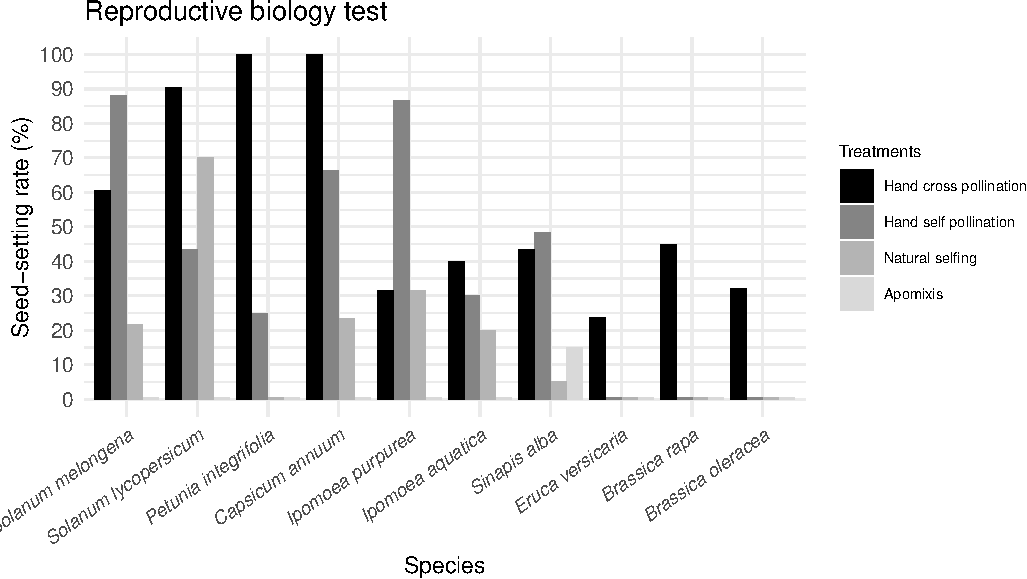
\includegraphics{output/figures/unnamed-chunk-2-1.pdf}
\caption{The effect of heterospecific pollen (scaled see set) is
represented in function of the compatibility system (self/cross*100) for
the the different species. Each coulored dot represents the interaction
of a focal species with a different pollen donor.}
\end{figure}

\newpage

\section{DISCUSSION}\label{discussion}

Discussion

\begin{enumerate}
\def\labelenumi{\arabic{enumi}.}
\tightlist
\item
  What are the implications of the findings?
\end{enumerate}

\section{CONCLUSIONS}\label{conclusions}

\section{ACKNOWLEDGEMENTS}\label{acknowledgements}

\section{REFERENCES}\label{references}

\hypertarget{refs}{}
\hypertarget{ref-aizen2007}{}
Aizen, M. A., and L. D. Harder. 2007. Expanding the limits of the
pollen-limitation concept: Effects of pollen quantity and quality.
Ecology 88:271--281.

\hypertarget{ref-arceo2018}{}
Arceo-Gómez, G., C. Alonso, T.-L. Ashman, and V. Parra-Tabla. 2018.
Variation in sampling effort affects the observed richness of
plant--plant interactions via heterospecific pollen transfer:
Implications for interpretation of pollen transfer networks. American
journal of botany 105:1601--1608.

\hypertarget{ref-arceo2016}{}
Arceo-Gómez, G., and T.-L. Ashman. 2016. Invasion status and
phylogenetic relatedness predict cost of heterospecific pollen receipt:
Implications for native biodiversity decline. Journal of Ecology
104:1003--1008.

\hypertarget{ref-arceo2016can}{}
Arceo-Gómez, G., R. A. Raguso, and M. A. Geber. 2016. Can plants evolve
tolerance mechanisms to heterospecific pollen effects? An experimental
test of the adaptive potential in clarkia species. Oikos 125:718--725.

\hypertarget{ref-ashman2013}{}
Ashman, T.-L., and G. Arceo-Gómez. 2013. Toward a predictive
understanding of the fitness costs of heterospecific pollen receipt and
its importance in co-flowering communities. American Journal of Botany
100:1061--1070.

\hypertarget{ref-barrett1988}{}
Barrett, S. C. 1988. The evolution, maintenance, and loss of
self-incompatibility systems. Plant reproductive ecology: patterns and
strategies:98--124.

\hypertarget{ref-bartomeus2008}{}
Bartomeus, I., J. Bosch, and M. Vilà. 2008. High invasive pollen
transfer, yet low deposition on native stigmas in a carpobrotus-invaded
community. Annals of Botany 102:417--424.

\hypertarget{ref-bascompte2003}{}
Bascompte, J., P. Jordano, C. J. Melián, and J. M. Olesen. 2003. The
nested assembly of plant--animal mutualistic networks. Proceedings of
the National Academy of Sciences 100:9383--9387.

\hypertarget{ref-brown2001}{}
Brown, B. J., and R. J. Mitchell. 2001. Competition for pollination:
Effects of pollen of an invasive plant on seed set of a native congener.
Oecologia 129:43--49.

\hypertarget{ref-carvalheiro2014}{}
Carvalheiro, L. G., J. C. Biesmeijer, G. Benadi, J. Fründ, M. Stang, I.
Bartomeus, C. N. Kaiser-Bunbury, M. Baude, S. I. Gomes, V. Merckx, and
others. 2014. The potential for indirect effects between co-flowering
plants via shared pollinators depends on resource abundance,
accessibility and relatedness. Ecology letters 17:1389--1399.

\hypertarget{ref-engel2003}{}
Engel, E. C., and R. E. Irwin. 2003. Linking pollinator visitation rate
and pollen receipt. American Journal of Botany 90:1612--1618.

\hypertarget{ref-fang2013}{}
Fang, Q., and S.-Q. Huang. 2013. A directed network analysis of
heterospecific pollen transfer in a biodiverse community. Ecology
94:1176--1185.

\hypertarget{ref-galen1989}{}
Galen, C., and T. Gregory. 1989. Interspecific pollen transfer as a
mechanism of competition: Consequences of foreign pollen contamination
for seed set in the alpine wildflower, polemonium viscosum. Oecologia
81:120--123.

\hypertarget{ref-inouye1980}{}
Inouye, D. W. 1980. The terminology of floral larceny. Ecology
61:1251--1253.

\hypertarget{ref-lloyd1992}{}
Lloyd, D. G., and D. J. Schoen. 1992. Self-and cross-fertilization in
plants. i. functional dimensions. International Journal of Plant
Sciences 153:358--369.

\hypertarget{ref-montgomery2012}{}
Montgomery, B. R., and B. J. Rathcke. 2012. Effects of floral
restrictiveness and stigma size on heterospecific pollen receipt in a
prairie community. Oecologia 168:449--458.

\hypertarget{ref-morales2008}{}
Morales, C. L., and A. Traveset. 2008. Interspecific pollen transfer:
Magnitude, prevalence and consequences for plant fitness. Critical
Reviews in Plant Sciences 27:221--238.

\hypertarget{ref-neiland1999}{}
Neiland, M., and C. Wilcock. 1999. The presence of heterospecific pollen
on stigmas of nectariferous and nectarless orchids and its consequences
for their reproductive success. Protoplasma 208:65--75.

\hypertarget{ref-pauw2013}{}
Pauw, A. 2013. Can pollination niches facilitate plant coexistence?
Trends in ecology \& evolution 28:30--37.

\hypertarget{ref-R_Core_Team_2018}{}
R Core Team. 2018. R: A language and environment for statistical
computing. R Foundation for Statistical Computing, Vienna, Austria.

\hypertarget{ref-thomson1982}{}
Thomson, J. D., B. J. Andrews, and R. Plowright. 1982. The effect of a
foreign pollen on ovule development in diervilla lonicera
(caprifoliaceae). New Phytologist 90:777--783.

\hypertarget{ref-tong2016}{}
Tong, Z.-Y., and S.-Q. Huang. 2016. Pre-and post-pollination interaction
between six co-flowering pedicularis species via heterospecific pollen
transfer. New Phytologist 211:1452--1461.

\hypertarget{ref-whitehead2018}{}
Whitehead, M. R., R. Lanfear, R. J. Mitchell, and J. D. Karron. 2018.
Plant mating systems often vary widely among populations. Frontiers in
Ecology and Evolution 6:38.

\eleft

\clearpage

\listoftables

\newpage

\newpage

\clearpage

\listoffigures

\newpage

\newpage

\blandscape

\elandscape

\clearpage

\end{document}